\section{Introduction}

Much work has been done on the topic of \emph{data provenance}, which aims to provide
transparency in data analytics systems by allowing a user to interrogate where data has come
from, the ways it has been manipulated and transformed. Collecting such information
requires a lot of effort, work has gone into integrating data provenance features
into programming languages themselves \cite{fehrenbach16}. More recent work
extends this approach to work with data visualizations \cite{perera22}.

Provenance information is of great utility in science communication: good science is
\emph{reproducible}, and good science communication should give the layperson as many tools
as possible to verify or reproduce conclusions made from data.

Communication is often done through combining the mediums of text,
data visualizations, and code. The idea of literate programming \cite{knuth84} has
been influential, and in data analytics the ``notebook interface'' \cite{kluyver16}, is popular
allowing a data scientist to interleave code with its own results, and expository text. 

\begin{figure}[h]
   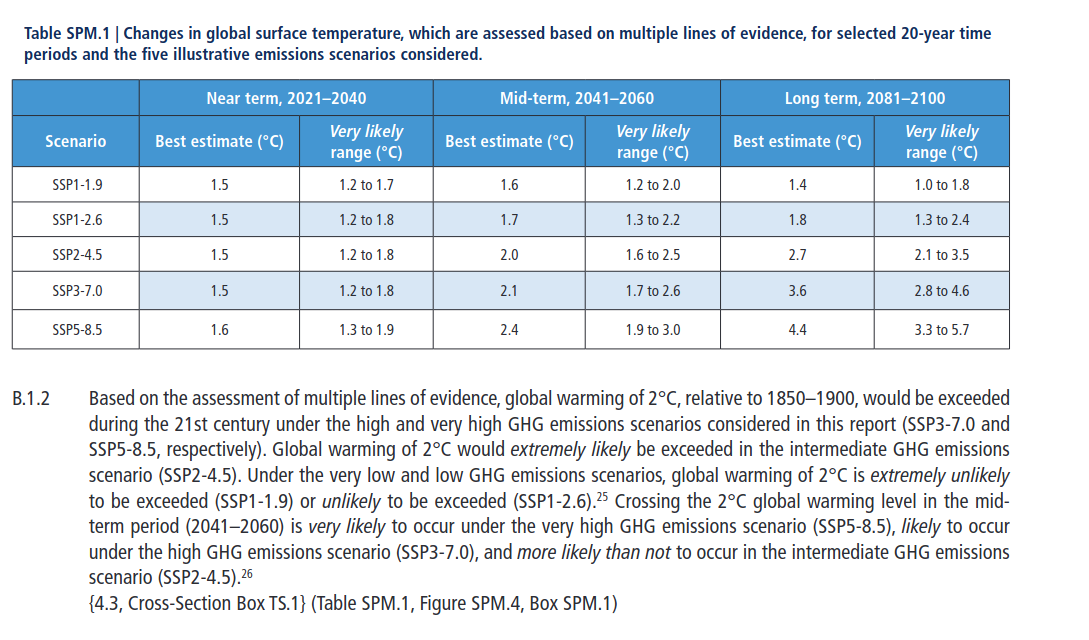
\includegraphics[width=0.7\textwidth]{fig/ipcc-table-explanation.png}
   \caption{Explanation suported by contents of table}
   \label{fig:table-explanation}
\end{figure}

Whilst these solutions provide some level of transparency, they come with limitations. Users do not want to 
install bespoke software in order to read articles, and notebooks do not necessarily provide complete
transparency by themselves; the code is often highly abstract, providing wrappers
for complex models which have often been applied as black-boxes.

More recently, \cite{dragicevic19} proposed the idea of an \emph{explorable multiverse} as a
mechanism for improving transparency. The idea is that during data analysis, choices made by
the analyst can significantly impact results; and that analysis should be run multiple times
using different methods. The user should then be allowed to toggle between different choices
and see how a change in the method impacts the conclusions that can be drawn from the data.

\cite{psallidas18} has done work on applying techniques of data lineage to interactive
visualizations based on in-memory databases. Their work allows for fine-grained
provenance queries at high-speed, but does not extend this work to supporting text.
In general it is unclear what a data provenance query on text looks like, or how one
might write an article as a program that allows for interactive provenance queries on text.

Whilst we do not propose to solve the problem of deliberate misinformation,
interactive features, which allow readers to interrogate where data came from and how
it was used to support an argument, allow both laypeople and policymakers to make more
informed decisions. Increased data transparency is a good thing. Transparency
should not be considered a binary quantity. Instead it is helpful to think of it as a continuum.

A traditional computer program is often less transparent than one presented as a notebook,
similarly, a paper that does not come with an artifact is less transparent than if the artifact
was included. A programming language with data provenance is more transparent than one without.
Increasing transparency is useful, but science communication may never be fully transparent.
Unfortuantely, we cannot stop malicious actors from misusing data, nor force them to use transparent
systems, but we believe that the ideas demonstrated in this proposal will go some way
to improving the situation.

To meet this goal, we need to allow authors to introduce a richer kind of reference into supporting
text. Making reference to visual marks or underlying data can be thought of as a \emph{query},
interacting with a textual reference should query the underlying data, and provide the user with immediate
visual feedback, perhaps by highlighting elements of relevant visualizations, perhaps by showing the user
how a given result was computed. We stress that generic tooling for this sort of thing does not yet exist.
We call text that comes with an account of how it was generated \emph{self-certifying text}.

\begin{figure}
   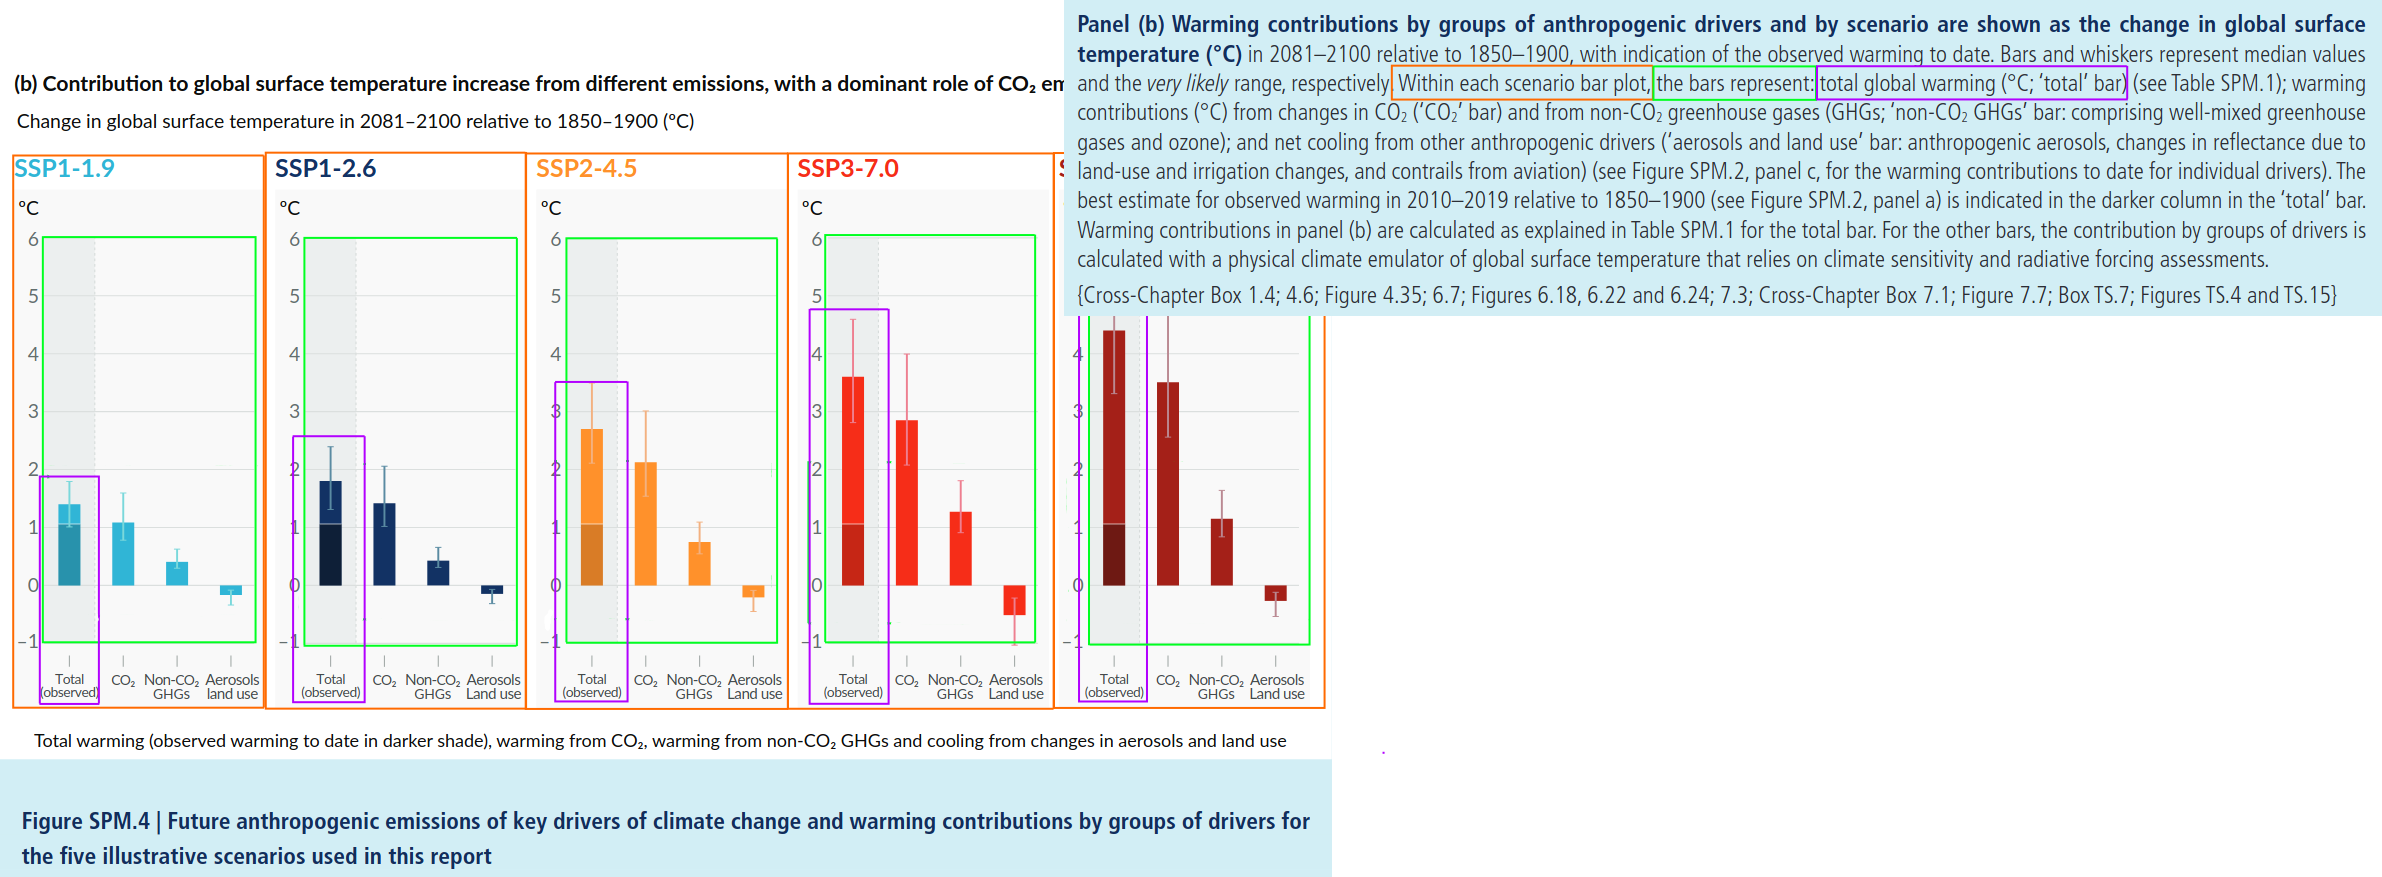
\includegraphics[width=0.9\textwidth]{fig/ipcc-visual-elements.png}
   \caption{Examples of scope in linked text}
   \label{fig:visual-element-scope}
\end{figure}

\subsection{Self-Certifying Text}
What does it mean for supporting text to be self-certifying? 

\subsubsection{Quantitative Expressions}
\begin{itemize}
   \item Raw results
   \item percentages
   \item rounded or normalized information
\end{itemize}
% Directly embedding a quantitative expression into the text seems to be the simplest
% of the linguistic categories we have identified thus far, but this may not be the case. Embedding
% a percentage may be simple: requiring the user to only provide a numerical value, and scaling it
% to be in the range of $0$-$100$, but more complicated expressions, such as a description of a calculation
% may be more difficult to synthesize. Solving the problem of explaining a calculation or piece of a program
% will itself go a long way to improving the transparency of a piece of science communication.

\subsubsection{Graded Adjectives}
A graded adjective is an adjective that can be modified to make its form stronger or weaker.
As an example, consider mapping ranges of probabilities onto natural language. If the probability
of an event occurring is $1$, we can say it is \emph{certain} to occur. If instead it is $0.99$
or some other value arbitrarily close to $1$, we will \emph{grade} the adjective to weaken it:
it is \emph{virtually certain} to occur. We see examples of this in \figref{table-explanation},
with the terms ``exceptionally unlikely'' and ``virtually certain''.

% Considered in more depth, we arrive at the concept of modalities in natural language. Similar to 
% the concepts in modal logic, a modality allows the expression of concepts such as necessity or possibility.
% In the context described above, the idea that a probability is \emph{virtually certain} introduces the modality of
% possibility -- an event must be possible in order to be virtually certain to occur. Even something simple
% like the discussion of probabilities above can combine the two into the idea of graded modality:
% if something is ``very likely'', we would still believe that it is less likely to occur than something that
% is ``virtually certain''. Handling these sorts of linguistic constructs will be a key part of addressing
% the problem. 

\subsubsection{Selecting Visual Elements: Iteration, Scope and Mereology}
Text that refers to objects of discourse is relatively common, but even direct references are non-trivial 
linguistically. \figref{visual-elements-scope} -- taken from \cite{lee23} -- shows an example \textit{in situ},
the report it is taken from collates a large amount of climate research data, and attempts to synthesize
useful information for policymakers. Even this simple example shows the complexity of the problem: the text highlighted
in orange refers to the collection of bar-charts shown on the left hand side, introducing a set of 5 bar-charts
into the scope of discourse. The text highlighted in green refers to the bars within these charts, mapping 
a narrowing of scope across the bar-charts that have already been introduced. Then, the text highlighted in
purple narrows this scope further to talk about the bar representing total warming, again within each of the
charts at the same time. To handle this kind of reference, we need a generic mechanism for referencing
containers independently of their contents.

% This illustrative example showcases several sub-problems our system will need to be able to handle. First
% is that of creating an iterative scope for the references that follow. We can imagine that the orange-highlighted
% text effectively creates an iterable, which the green highlighted text maps over. The purple-highlighted text
% then maps over the iterable created by the green highlighted text. This sort of iteration is a common feature of natural language,
% and any well-designed system should allow for such expressions to be written by the author, and linked appropriately.

% In order to reference common substructures that appear within the 5 charts, the system must be able to walk arbitrarily 
% into structured data objects. In linguistics this is referred to as ``mereology'', the study of relationships
% between parts and wholes. In our case, one could imagine the collection of 5 charts as the whole, with each
% individual bar-chart being a part of that whole. Because all 5 charts are structurally the same (of the same type),
% we can apply the same walk to each of them: bar-charts in our language have a field called \kw{bars}, a list
% of the various bars. In this light, we can imagine the green-highlighted text as walking into the \kw{bars} field
% of the charts, and the purple-highlighted text as walking into this list, and selecting the bar with the label "total warming".

